% title: figs.tex
% description: 
% author: twab

\begin{figure}[h] %% figure [x] -- impute.pdf
  \begin{fullwidth}
  \begin{center}
	  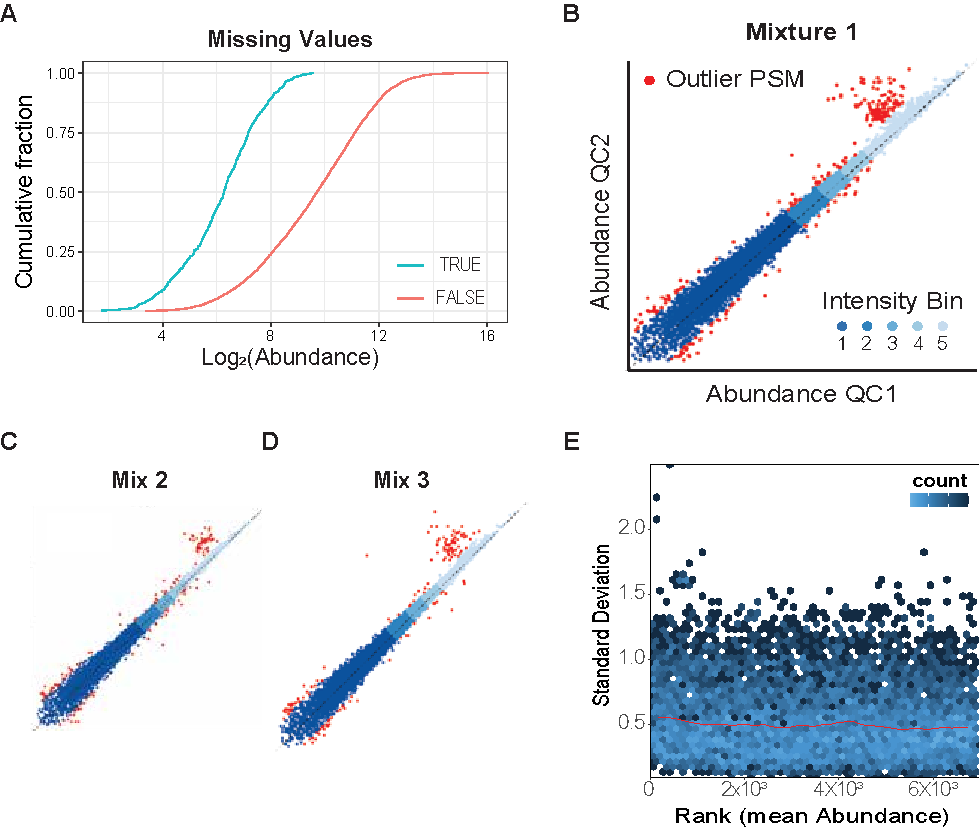
\includegraphics[width=0.9\paperwidth,keepaspectratio]{impute}
	  \caption{\textbf{Missing value imputation and PSM outlier removal.}
	  \textbf{A} \textbf{B} \textbf{C} \textbf{D} }
	  \label{fig:impute}
  \end{center}
  \end{fullwidth}
\end{figure}


\begin{figure}[h] %% figure [x] -- normalization.pdf
  \begin{fullwidth}
  \begin{center}
	  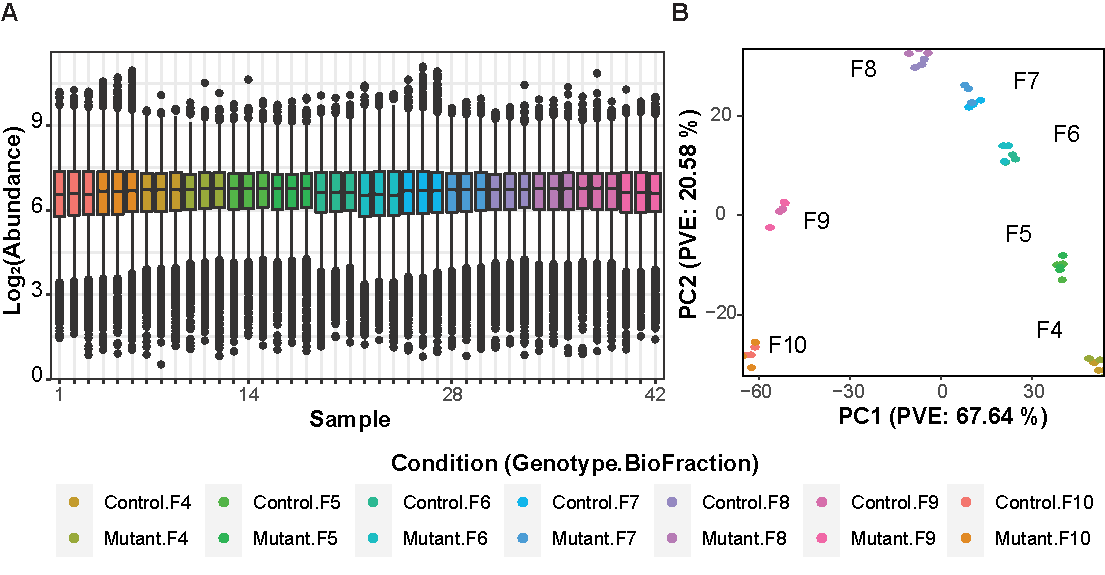
\includegraphics[width=0.9\paperwidth,keepaspectratio]{normalization}
	  \caption{\textbf{Data Normalization and PCA.} \textbf{A} \textbf{B} }
	  \label{fig:normalization}
  \end{center}
  \end{fullwidth}
\end{figure}


\begin{figure}[h] %% figure [x] -- washc4.pdf
  \begin{fullwidth}
  \begin{center}
	  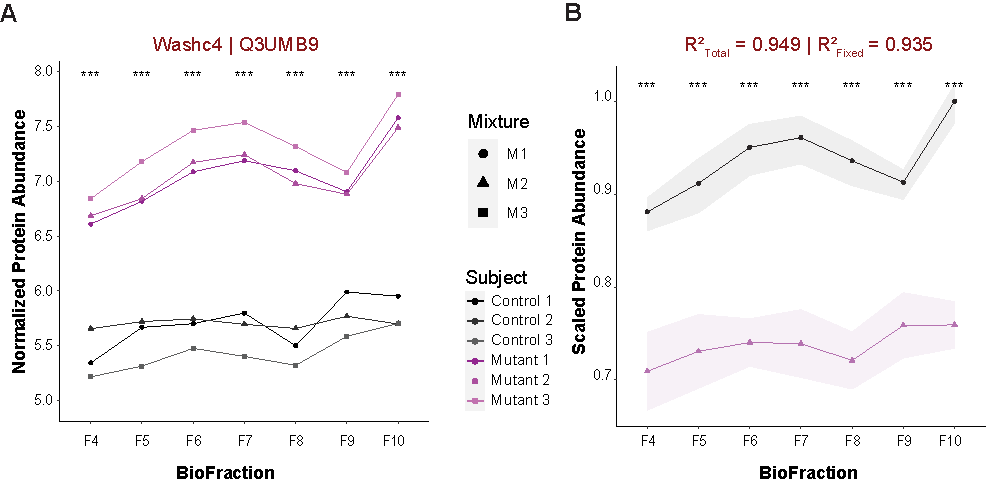
\includegraphics[width=0.9\paperwidth,keepaspectratio]{washc4}
	  \caption{\textbf{Data Normalization and PCA.} \textbf{A} \textbf{B} }
	  \label{fig:washc4}
  \end{center}
  \end{fullwidth}
\end{figure}


\begin{figure}[h] % figure -- gof
	\begin{fullwidth}
		\begin{center}
		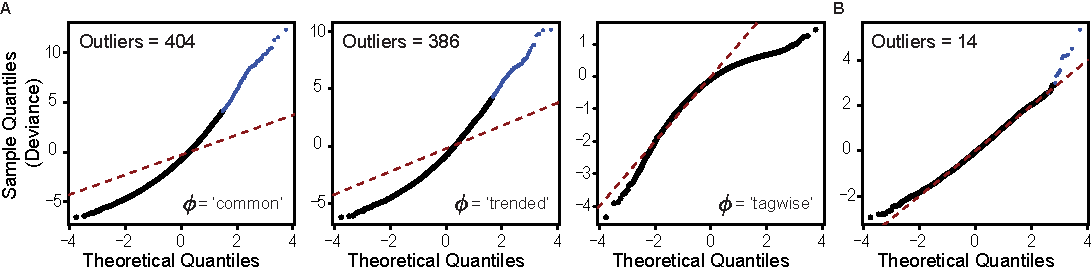
\includegraphics[width=0.9\paperwidth,keepaspectratio]{gof}
		\caption{\textbf{Goodness-of-fit of \texttt{edgeR} (A), and 
		\texttt{MSstatsTMT} (B) statistical approaches.} The overall
		adequacy of the linear models fit to the data were assessed 
		by plotting the residual deviance for all proteins as a 
		quantile-quantile plot (McCarthy \textit{et al.}, (2012)). 
		\textbf{(A)} For analysis with \texttt{edgeR}, The normalized
		protein data from \texttt{MSstatsTMT} were fit with a negative
		binomal generalized linear model of the form: 
		\texttt{Abundance} $\sim$ \texttt{Mixture + Condition}.
		Where \texttt{Mixure} is an additive blocking factor that 
		accounts for variablity between experiments. 
		The NB framework used by \texttt{edgeR} utilizes a dispersion 
			parameter 
		to account for mean-variance relationships in the data.
		The dispersion parameter can take several forms including:
                'common', 'trended', and 'tagwise'. We plot the deviance
		stattistics for the data fit with each of
		the three disperions parameters against their 
		theoretical normal quantiles using the \texttt{edgeR::gof}
		function. \textbf{(B)} For analysis with \texttt{MSstatsTMT},
		the normalized protein data were fit with a linear mixed-effects 
		model (LMM) of the form: 
		\texttt{Abundance} $\sim$ \texttt{0 + Condition + (1|Mixture)}. 
		Where \texttt{Mixture} represents the mixed-effect
		of \texttt{Mixture}. The residual deviance and degrees of 
		freedom were extracted from the fitted models, z-score
		normalized, and plotted as in (A). Proteins with a significantly 
		poor fit are indicated as outliers in blue 
		(Holm-adjusted P-value $<$ 0.05).}
		\label{fig:gof}
	\end{center}
	\end{fullwidth}
\end{figure}


\begin{figure}[h] %% figure x -- design 
  \begin{fullwidth}
  \begin{center}
	  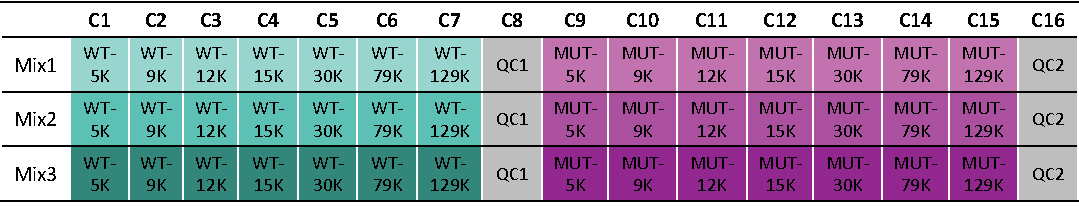
\includegraphics[width=0.9\paperwidth,keepaspectratio]{design}
	  \caption{\textbf{Experimental Design.} We performed three 16-plex TMT
	  experiments. Each TMT mixture is a concatenation of 16 labeled
	  samples. In each experiment we analyzed seven subcellular
	  \texttt{BioFractions} prepared from the brain of a single Control
	  and 'Mutant' mouse. In all, we analyzed three \texttt{Subjects} from 
	  each {Condition}. Each \texttt{Mixture} includes two \texttt{Channels}
	  dedicated to the analysis of a common quality control (QC) sample for
	  normalization between MS runs.}
	  \label{fig:design}
  \end{center}
  \end{fullwidth}
\end{figure}


\begin{figure}[h] %% figure x -- contrasts
  \begin{fullwidth}
  \begin{center}
	  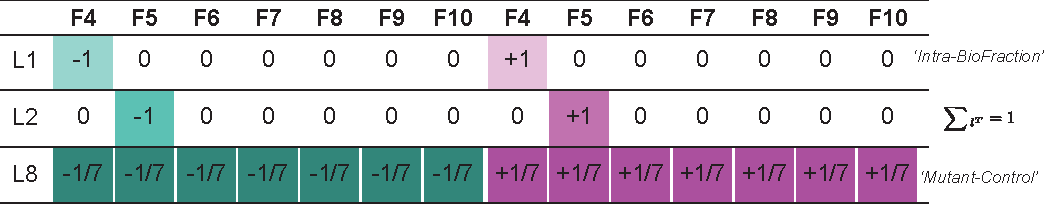
\includegraphics[width=0.9\paperwidth,keepaspectratio]{contrasts}
	  \caption{\textbf{Statistical Comparisons.} We assessed two types of
	  contrasts. Each row of the matrix specifies a contrast between
	  positive and negative coefficients in the mixed-effects model fit to
	  each protein. Contrasts1-7 are intra-BioFraction contrasts that
	  specify the pairwise comparisons of Control and Mutant groups for a
	  single fraction. In Contrast 8 we compare Mutant-Control and asses
	  the overall difference of Control and Mutant conditions.  Each
	  contrast is a vector of sum 1.}
	  \label{fig:contrasts}
  \end{center}
  \end{fullwidth}
\end{figure}


\begin{figure}[h] %% figure -- variance
  \begin{fullwidth}
  \begin{center}
	  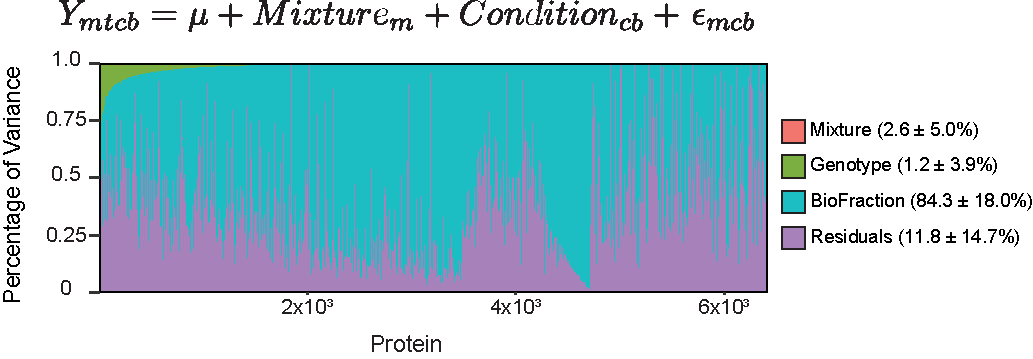
\includegraphics[width=0.9\paperwidth,keepaspectratio]{variance}
	  \caption{\textbf{Analysis of Variance Components.} 
	  The proportion of variance explained by Genotype, BioFraction,
	  Mixture, and remaining residual error (subplot error) for all
	  proteins. Note while the contribution of Mixture seems negligiable,
	  its average for all proteins is approximately twice the average
	  percent variance explained by Genotype. BioFraction explains the
	  majority of the variance for all proteins. Analysis done with
	  \texttt{variancePartition::calcVarPart}.}
	  \label{fig:variance}
  \end{center}
  \end{fullwidth}
\end{figure}
